% !TeX spellcheck = en_US
%\documentclass[preprint,authoryear]{elsarticle}
\documentclass[preprint]{elsarticle}
% sudo apt-get install -y texlive-publishers

\usepackage[left]{lineno}
\usepackage[latin1]{inputenc}
\usepackage[T1]{fontenc}
\usepackage{lmodern}
\usepackage{multirow}

\usepackage{lineno,hyperref}
\modulolinenumbers[5]

\usepackage[none]{hyphenat}

\usepackage{url}
\usepackage{booktabs}

\usepackage{tikz}
\usetikzlibrary{calc}
\usetikzlibrary{positioning}

\usepackage{mathtools}
\usepackage{amssymb}
\usepackage{amsthm}

\usepackage{caption}
\captionsetup{labelfont=bf}
\captionsetup{skip=0pt}

\usepackage{pgfplots}
\pgfplotsset{compat=newest}
\usepackage{algorithm}

\usepackage[noend]{algpseudocode}

\usepackage[margin=0.9in]{geometry}

\usepackage[normalem]{ulem}
%\usepackage{xcolor}

\newcommand{\Comentar}[1]{\State {\cmmt{#1}}}
\newcommand{\Break}{\State \textbf{break}}
\renewcommand{\Return}{\State \textbf{return}~}
\renewcommand{\algorithmicensure}{\textbf{Parameters:}}

\renewcommand\algorithmicthen{}
\renewcommand\algorithmicdo{}


\algblock{ForEach}{EndFor}
\algblock{ForDownTo}{EndFor}
\algblock{ForTo}{EndFor}

\newcommand{\Block}[1]{\State #1 \{}
\newcommand{\EndBlock}{\State \}}

\usepackage{scrextend}
\newcommand{\boldm}[1] {\mathversion{bold}#1\mathversion{normal}}
\newcommand{\round}[1]{\ensuremath{\lfloor#1\rceil}}
\usepackage{setspace}
\usepackage{array}
\usepackage{color, colortbl}
\definecolor{Gray}{gray}{0.9}
\hyphenation{cost-ef-fec-tive-ness}

\newcommand{\specialcell}[2][c]{%
	\begin{tabular}[#1]{@{}c@{}}#2\end{tabular}}

\usepackage{textcomp}
\usepackage{graphicx} 
\setlength{\fboxsep}{0.005pt}
\newcommand{\tmpframe}[1]{\fbox{#1}}

\journal{Computers \& Industrial Engineering}


\begin{document}

\section{Introduction}
\section{Related literature}
\section{Problem context and assumptions}
\section{The mathematical modeling}
\section{Solution strategy}
\section{Implementation and results}
\label{sec6}

\subsection{Results obtained}

In the tests performed, we used a 64-bit, 16GB, 3.6GHz, eight-core processor with {\it Linux Ubuntu 22.04.1 LTS 64-bit} as the operational system and {\it Python 3.10.4}\/ as the programming language. We also used the well-known solver {\it Gurobi}\/ (www.gurobi.com), version 9.5.2.

We ran Algorithm \ref{alg:main} in the 5 scenarios described in Table \ref{tab:scenarios}, considering 6 methods for node-by-node solution: Gurobi (see \ref{solver}), ACO, NMO, TS, GRASP, and {\it Shims} (Algorithm \ref{alg:shims}). In generating the items in each node, we consider 3 values for the parameter $surplus$. The results obtained for the function $f$, with the corresponding run time in seconds, are shown in Tables \ref{tab:20} ($surplus = 1.2$), \ref{tab:50} ($surplus = 1.5$) and \ref{tab:100} ($surplus = 2.0$). For each $method$, $scenario$\/ and $surplus$, 7 different instances were generated. Therefore, 105 tests (5 scenarios $\times$\/ 3 volumes $\times$\/ 7 instances) were performed for each method. 

The average values were presented for $f_{\pi}$\/ and, for the run time, the worst result obtained. To facilitate the comparison between the methods, we added a last column in these tables, where two values are indicated:
\begin{itemize}
	\item {\bf Normalized}: value between 0 and 1, which corresponds to the ratio between the sum of $f$\/ values obtained by the method in all scenarios and the sum of the best values obtained among all methods in all scenarios. The higher the value of {\bf Normalized}, the closer the method approached the best solutions found.
	\item {\bf Speed-up}: ratio of the sums of the worst run times of all scenarios and the sum of the method run times in all scenarios. The method with the highest {\bf Speed-up}\/ is the fastest.
\end{itemize}

In each $scenario$\/, we indicate in bold the best value of $f$\/ found. In each table, we also indicate in bold the best {\bf Normalized}\/ and {\bf Speed-up}\/ values.

{\color{blue}
{\bf run time (s)} is the average time to solve a problem instance.

As the MIP solver was not capable of solving all scenarios in polynomial time or reached the computer's Read-Access Memory (RAM, 16 GiB) too early, we decided to set the Gurobi {\it MIPgap} parameter to 1\% to control the minimal quality of the returned solutions and abbreviate the solution time.
From now on, we will refer to this Gurobi-specific model as {\it Gurobi* }.
For more details on the Gurobi {\it MIPgap}, refer to \cite{mipgap}.

This decision hinders the MIP solver from reaching optimal solutions in favor of the possibility of result comparisons with the {\it Shims} heuristic.

}

\begin{table}[H]
\centering
\caption{Solutions with volume {\color{red}$surplus =1.2$} and 3600s as time limit.}  \label{tab:20}
\footnotesize
\begin{tabular}{ccccccccc}
\toprule
{\bf Tours}&$method$          & {\bf Scenarios} & {\bf 1} & {\bf 2} & {\bf 3} & {\bf 4} & {\bf 5} & \specialcell{{\bf Normalized}\\{\bf Speed-up}}   \\
\toprule
\multirow{4}{*}{ \specialcell{$\pi_{TSP_1}$\\ $\pi_{TSP_2}$ }} &\multirow{2}{*}{\it Gurobi* } & $f$ & 8.52    & 11.70   & 13.07   & 13.54 & 12.44     &  1.00\\ % 5927
&&               {\bf run time (s)}  & 17      & 17       & 16      & 17   & 26        &  1.0 \\ % 93
\cmidrule(lr){2-9}	
&\multirow{2}{*}{\it Shims}    & $f$ & 7.83    & 11.34   & 12.77   & 13.20 & 12.22     &  0.97 \\ % 5736
&&         {\bf run time (s)}        & 4       & 5       &  6      & 7     & 10        &  2.9  \\ % 32

\midrule

\multirow{4}{*}{\it $S_{K}$ }&\multirow{2}{*}{\it Gurobi* } & $f$ & 8.51    & 12.25   & 13.32   & 14.61  & x        & 1.00 \\ % 4869
&&               {\bf run time (s)}  & 25      & 36      & 121     & 297    & x        &  1.0 \\ % 479
\cmidrule(lr){2-9}	
&\multirow{2}{*}{\it Shims}    & $f$ & 8.11    & 12.18   & 13.25   & 14.57  & 14.33    &  0.99 \\ % 4811
&&         {\bf run time (s)}        & 4       & 8       & 33      & 95     & 572      &  3.4  \\ % 140
\bottomrule
\multicolumn{9}{c}{*{\it MIPgap} parameter set to 1\%. The $f$ values are \textpm 1\% distant from the optimal solution}\\

\end{tabular}
\normalsize
\end{table}

{\color{blue}

97\% of 16GiB was the RAM state before we aborted the {\it Gurobi*} execution on solving scenario 5 in Table \ref{tab:20}.

}

\begin{table}[H]
	\centering
	\caption{Solutions with volume {\color{blue}$surplus=1.5$} and 3600s as time limit.}  \label{tab:50}
	\footnotesize
	\begin{tabular}{ccccccccc}
		\toprule
		{\bf Tours} & $method$          & {\bf Scenarios} & {\bf 1} & {\bf 2} & {\bf 3} & {\bf 4} & {\bf 5} & \specialcell{{\bf Normalized}\\{\bf Speed-up}}   \\
		\toprule
		\multirow{4}{*}{ \specialcell{$\pi_{TSP_1}$\\ $\pi_{TSP_2}$ }} & \multirow{2}{*}{\it Gurobi* } & $f$ & 11.80 & 16.74 & 18.04 & 18.86 & 16.92 & 1.00 \\ % 8236
		&&               {\bf run time (s)}  & 38    & 30    & 27    & 29    & 81    & 1.00  \\ % 205
		\cmidrule(lr){2-9}	
		&\multirow{2}{*}{\it Shims}    & $f$ & 10.89 & 16.65 & 17.80 & 18.69 & 16.45 & 0.98  \\ % 8048
		&&         {\bf run time (s)}        & 4     & 5     & 6     & 7     & 8     & 7.1   \\ % 29
		
		\midrule
		
		\multirow{4}{*}{\it $S_{K}$ } & \multirow{2}{*}{\it Gurobi* } & $f$ & 11.81 & 17.01 & 18.25 & 20.59 & 18.36   & 1.00 \\ % 8602
		&&               {\bf run time (s)}  & 53    & 61    & 193   & 470   & 2241    & 1.0  \\ % 3018
		\cmidrule(lr){2-9}	
		&\multirow{2}{*}{\it Shims}    & $f$ & 11.33 & 16.97 & 17.56 & 20.43 & 17.94   & 0.98  \\ % 8423
		&&         {\bf run time (s)}        & 4     & 8     & 34    & 96    & 591     & 4.1 \\ % 733
		\bottomrule
	
	\end{tabular}
	\normalsize
\end{table}


\begin{table}[H]
	\centering
	\caption{Solutions with volume {\color{violet}$surplus=2.0$} and 3600s as time limit.}  \label{tab:100}
	\footnotesize
	\begin{tabular}{ccccccccc}
		\toprule
		{\bf Tours} & $method$          & {\bf Scenarios} & {\bf 1} & {\bf 2} & {\bf 3} & {\bf 4} & {\bf 5} & \specialcell{{\bf Normalized}\\{\bf Speed-up}}   \\
		\toprule
		\multirow{4}{*}{ \specialcell{$\pi_{TSP_1}$\\ $\pi_{TSP_2}$ }} & \multirow{2}{*}{\it Gurobi* } & $f$ & 17.75 & 24.39 & 26.46 & 27.09 & 24.00 & 1.00 \\ % 119.69
		&&                                                                               {\bf run time (s)}  & 162   & 95    & 74    & 68    & 67    & 1.0  \\ % 466
		\cmidrule(lr){2-9}	
		&                                                                   \multirow{2}{*}{\it Shims} & $f$ & 16.73 & 24.06 & 26.15 & 26.25 & 23.54 &  0.97 \\ % 116,48
		&&                                                                                {\bf run time (s)} & 5     & 6     & 8     & 10    & 11    &  11.7  \\ % 40
		
		\midrule
		
		                                 \multirow{4}{*}{\it $S_{K}$ } & \multirow{2}{*}{\it Gurobi* } & $f$ & 17.75 & 25.24 & 26.46 & 29.11 &  x   & 1.00 \\ % 9856
		&&                                                                                {\bf run time (s)} & 151   & 123   & 319   & 689   &  x   & 1.0  \\ % 1282
		\cmidrule(lr){2-9}	
		&                                                                \multirow{2}{*}{\it Shims}    & $f$ & 16.88 & 24.30 & 26.24 & 28.65 & 28.74 & 0.97  \\ % 9607
		&&                                                                                {\bf run time (s)} & 5     & 9     & 37    & 108   & 625   & 8.1  \\ % 159
		\bottomrule
		
	\end{tabular}
	\normalsize
\end{table}

{\color{blue}
{\it Gurobi*} could not solve scenario 5 in Table \ref{tab:100} because $3600/K! = 0.71s$, not enough time for {\it Gurobi*} to find a feasible node solution.
}

\subsubsection{Time limits comparisons}

\begin{table}[H]
	\centering
	\caption{Solutions with different time limitations for $S_K$ tours.}  \label{tab:100time}
	\footnotesize
	\begin{tabular}{ccc|cc|cc|cc}
		\toprule
		&             \multicolumn{2}{r}{\bf Volume $surplus$} &\multicolumn{2}{c}{$1.2$}&\multicolumn{2}{c}{$1.5$}&\multicolumn{2}{c}{$2.0$} \\
		\midrule
$method$& {\bf \specialcell{Time\\limit (s)}} & {\bf Scenarios}    & {\bf 4} & {\bf 5} & {\bf 4} & {\bf 5} & {\bf 4} & {\bf 5} \\
		\toprule
		
		\multirow{6}{*}{\it Gurobi* }& \multirow{2}{*}{1200} & $f$ & 14.67   & x       &  20.64  &  x      & 27.97   & x \\ % 
		&        &  {\bf run time (s)}                             & 217     & x       &  304    &  x      & 579     & x \\ % 
		\cmidrule(lr){2-9}                              
		& \multirow{2}{*}{2400}& $f$                               & 14.59   & 13.59   &  20.60  &  x      & 29.10   & x \\ % 
		&        &  {\bf run time (s)}                             & 313     & 1460    &  327    &  x      & 543     & x \\ % 
		\cmidrule(lr){2-9}                              		
		& \multirow{2}{*}{3600}& $f$                               & 14.61   & x       &  20.59  & 18.36   & 29.11   & x \\ % 
		&        &  {\bf run time (s)}                             & 297     & x       &  470    & 2241    & 689     & x \\ % 		
		\midrule
		\multirow{6}{*}{\it Shims}   & \multirow{2}{*}{1200} & $f$ & 15.14   &         &         &         &         &   \\ % 
		&        & {\bf run time (s)}                              & 73      &         &         &         &         &   \\ % 
		\cmidrule(lr){2-9}                              
		& \multirow{2}{*}{2400}& $f$                               &         &         &         &         &         &   \\ % 
		&        &  {\bf run time (s)}                             &         &         &         &         &         &   \\ % 	
		\cmidrule(lr){2-9}                              
		& \multirow{2}{*}{3600} & $f$                              & 14.57   & 14.33   &  20.43  & 17.94   & 28.65   & 28.74 \\ %  
		&        &  {\bf run time (s)}                             &  95     &  572    &  96     & 591     & 108     &  625  \\ %  	                                        
		\bottomrule
		
	\end{tabular}
	\normalsize
\end{table}


\begin{figure}[H]
\centering
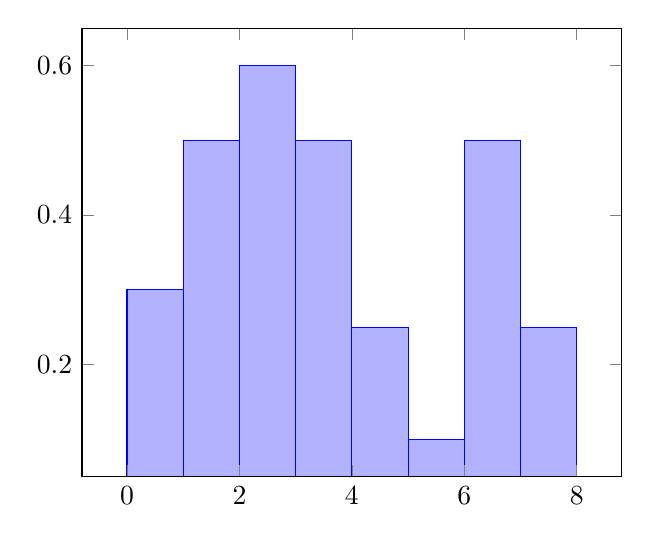
\begin{tikzpicture}
	\begin{axis}[
		area style,
		]
		\addplot+[ybar interval,mark=no] plot coordinates { 
			(0,.3)
			(1,.5)
			(2,.6)
			(3,.5)
			(4,.25)
			(5,.1)
			(6,.5)
			(7,.25)
			(8,.1)
		};
	\end{axis}
\end{tikzpicture}
\captionof{figure}{ESTE GR�FICO � APENAS UM MODELO}
\end{figure}




{\color{blue}

\subsubsection{Proposed K! strategy assessment}

Another important test is to compare the best tour score/cost ratio with the least expensive tour score/cost ratio. This is important to see how far our solution strategy is from the simplest form, just solving a TSP.

For this achievement, we ran {\it Shims} in 5 scenarios with 7 instances each, and 3 volume surpluses, collecting the averages of the best tour result and the least cost tour result.

\begin{table}[H]
\centering
\caption{{\it Shims} best and least cost tour results}  \label{tab:20least}
\footnotesize
\begin{tabular}{ccccccccc}
\toprule
{$surplus$}              & {\bf Tour} & {\bf 1} & {\bf 2} & {\bf 3} & {\bf 4}  & {\bf 5}   & {\bf Sum} & {\bf Improvement}\\
\toprule

\multirow{2}{*}{$1.2$}   & Least cost    & 7.83    & 11.34 & 12.77 & 13.20 & 12.22  & 57.36 &       \\ 
                         & Best in $K!$  & 8.11    & 12.18 & 13.25 & 14.57 & 14.33  & 62.44 & 8.9\%  \\ 
\midrule[.1pt]	
\multirow{2}{*}{$1.5$}   & Least cost    & 10.89   & 16.65 & {\color{red}17.80} & 18.69 & 16.45  & 80.48 & \\ 	
                         & Best in $K!$  & 11.33   & 16.97 & 17.56 & 20.43 & 17.94  & 84.23 & 4.8\%  \\ 
\midrule[.1pt]	
\multirow{2}{*}{$2.0$}   & Least cost    & 16.73   & 24.06 & 26.15 & 26.25 & 23.54  & 116.73&  \\ 
                         & Best in $K!$  & 16.88   & 24.30 & 26.24 & 28.65 & 28.74  & 124.81& 6.7\%   \\ 		                         
\midrule[.1pt]
\multicolumn{8}{r}{{\bf K! strategy advantage}}                                              & {\bf 6.8}\% \\

\bottomrule
\end{tabular}
\normalsize
\end{table}

As the selection of the best tour, considering what was collected and delivered in each node, and considering the cost increase due to CG deviation, was better than the option for a simple TSP solution (\textit{Least cost} results), this confirms that our solution strategy was adequate.

It is important to report that the best tour found in each test was seldom the tour with the lowest cost (the minimal cost tour without considering the CG deviation), but any of the first 25\% of the best tours. This indicates that our strategy of enumerating and solving all tours was assertive, although it is possible to devise a more proactive strategy to discard most of the higher-cost tours and improve performance. This must be one of the next steps in this research.

If a posterior application of this method requires 8, 9, or more nodes, it is possible to use this 25\% as a threshold to discard the higher-cost tours and keep the run time within an operational acceptable limit for the client.

\subsubsection{Final considerations on the results}

Most of the {\it Gurobi*} executions consumed over 12 GiB in total, and considering that the computer used in the experiments has a standard RAM consumption when idle of 3.5 GiB (with the Python Interface Development Environment (IDE), a PDF viewer, a system monitor, and a {\it LaTeX} IDE simultaneously open), the actual RAM consumption of {\it Gurobi*} was over 8.5 GiB.

All {\it Shims} executions consumed at most 1.5 GiB, requiring 5 GiB of total memory.
These details are important for a future application to adequately dimension the computer to be used.

}

\begin{thebibliography}{00}
	
	\bibitem{mipgap} Matthias Miltenberger. {\it What is the MIPGap?} \url{https://support.gurobi.com/hc/en-us/articles/8265539575953-What-is-the-MIPGap-}, 2023.
	
\end{thebibliography}


\end{document}
